\section{Ainul Filiani 1174073}
\subsection{Pengertian Kecerdasan Buatan}
kecerdasan buatan adalah salah satu cabang ilmu pengetahuan yang berhubungan dengan mesin untuk memecahkan persoalan yang rumit dengan cara yang lebih manusiawi. Hal ini biasanya dilakukan dengan mengikuti karakteristik dan anologi berpikir dari kecerdasan  atau inteligance manusia, dan menerapkan sebagai algoritma yang dikenal oleh komputer.
Dengan suatu pendekatan yang kurang lebih fleksibilitas dan efisien dapat diambil tergantung keperluan yang mempengaruhi bagaimana wujud dari prilaku kecerdasan buatan. AI biasanya dihubungkan dengan ilmu komputer, akan tetapi juga terkait erat dengan bidang lain seperti matematika, Psikologi, Pengamatan, Biolog, filosofi, dan lainnya
\subsection{Sejarah Kecerdasan Buatan}
Kecerdasan buatan merupakan bidang ilmu komputer yang sangat penting di era kini dan masa yang akan datang untuk mewujudkan sistem komputer yang cerdas. Bidang ini telah berkembang sangat pesat di 20 tahun terakir seiring dengan kebutuhan perangkat cerdas pada industry dan rumah tangga.
Kata Intelligance berasal dari bahasa latin "intelligo" yang berarti "saya paham". Berarti dasar dari intelligance adalah kemampuan untuk memahami dan melakukan aksi. nyatanya, bidang Kecerdasan Buatan atau disingkat dengan AI, berawal dari kemunculan komputer sekitar tahun 1940-an, sedangkan perkembangan sejarah dapat ditelusuri sejak zaman Mesir kuno. Pada saat ini, perhatian mendesak diberikan pada kemampuan komputer untuk melakukan hal-hal yang dapat dilakukan manusia. Dalam hal ini, komputer ini dapat meningkatkan kemampuan kecerdasan dan kecerdasan manusia.
Pada awal abad ke-17, René berbicara tentang tubuh binatang yang tidak meminta apa pun selain mesin yang rumit. Blaise Pascal membuat mesin hitung digital mekanis pertama pada tahun 1642. Pada 19, Charles Babbage dan Ada Lovelace bekerja pada mesin hitung mekanis yang dapat diprogram. Bertrand Russell dan Alfred Whitehead North menerbitkan Principia Mathematica, yang merombak logistik formal. Warren McCulloch dan Walter Pitts menerbitkan "Kalkulus Logika Gagasan yang Menjaga Aktivitas" pada tahun 1943 yang membentuk dasar bagi jaringan saraf.
1950-an adalah periode upaya aktif dalam AI. program permainan catur yang ditulis oleh Dietrich Prinz. John McCarthy menciptakan istilah "kecerdasan buatan" pada konferensi pertama yang menjadi dasar perjanjian itu, pada tahun 1956. Dia juga menemukan bahasa pemrograman Lisp. Alan Turing memperkenalkan "tes Turing" sebagai cara untuk mengoperasionalkan tes kecerdasan cerdas. 
\subsection{Perkembangan dan Penggunaan Kecerdasan}
Menurut studi Harvard Business Review dan ICM Unlimited pada tahun 2016, perusahaan besar memberikan kompensasi 10 persen lebih tinggi untuk setiap karyawan, Terrelong melanjutkan pengembangan Artificial Intelligence (AI) tidak hanya untuk membuat gambar atau video palsu lebih mudah, tetapi juga membuatnya sulit untuk membuktikan materi.Meskipun pada saat ini, upaya untuk membuat dan mendistribusikan konten hoax, alias hoaks, masih dapat diatasi, tetapi berhasil, tantangan yang dihadapi semakin sulit. Selain itu, AI memungkinkan pembuatan gambar, video, atau audio palsu dari bahan yang relatif minim.Moody's, yang harus disetujui, membuktikan upaya itu akan semakin menantang dan membutuhkan teknik forensik yang lebih canggih.Pada Mei 2019, para peneliti di Samsung AI Center dan Institut Sains dan Teknologi Skolkovo di Moskow, Rusia menunjukkan bahwa mereka dapat membuat tayangan video yang menampilkan masing-masing individu. Video ini sangat realistis tetapi sebenarnya palsu, dibuat menggunakan model pembelajaran tertentu yang disebut Generative Adversarial Network (GAN).Hasil dari proses GAN disebut deepfakes karena mereka menggunakan teknik pembelajaran yang mendalam untuk membuat konten palsu.Untuk jangka pendek, perusahaan diharapkan untuk terus memainkan media sosial dan situs untuk melihat pentingnya disinformasi dan meminta mereka yang bertanggung jawab untuk media sosial dan situs terkait untuk mengunduh konten.Terrelonge menambahkan langkah lain yang bisa diambil untuk merilis materi resmi untuk melawan konten palsu."Perlawanan terhadap konten palsu membutuhkan kombinasi teknologi dan pendidikan,".
\section{resume mengenai definisi supervised learning, klarifikasi, regresi, dan un-supervised learning. Data Set, training set dan testing set}
\subsection{Sipervised Learning}Supervised Learning adalah tugas mengumpulkan data untuk melengkapi fungsi data pelatihan yang diberi label. Data pelatihan terdiri dari contoh pelatihan. Dalam pembelajaran terawasi, setiap contoh adalah pasangan yang terdiri dari objek input (biasanya vektor) dan nilai output dingin (juga disebut sinyal pengawasan super). Algoritma pembelajaran yang diawasi menganalisis data pelatihan dan menghasilkan fungsi yang lengkap, yang dapat digunakan untuk memetakan contoh-contoh baru. Skenario  akan memungkinkan algoritma menentukan lable kelas dengan benar untuk instance yang tidak terlihat. Ini membutuhkan algoritma pembelajaran untuk menggeneralisasi data pelatihan sehingga tidak muncul dengan cara yang "masuk akal". Pembelajaran terawasi semakin dekat di mana ada pelatihan praktis selain dapat bervariasi yang berarti tujuannya adalah di mana mengelompokkan data ke dalam database yang ada. Pembelajaran terawasi menyediakan jumlah pembelajaran yang direkomendasikan untuk mendukung penilaian di masa depan. Obrolan, program mengemudi mandiri, pengenalan wajah, tatap muka dan robot adalah beberapa sistem yang dapat menggunakan pembelajaran yang diawasi atau tidak diawasi. Pembelajaran terbimbing sebagian besar terkait dengan AI berdasarkan pengambilan mereka juga mungkin diperlukan menggunakan model pembelajaran generatif. Pelatihan data untuk pembelajaran dimulai dengan mendiskusikan contoh-contoh dengan subjek input berpasangan dan output yang diinginkan (juga disebut sebagai sinyal pengawasan). Dalam pembelajaran yang diawasi untuk pemrosesan gambar, misalnya sistem AI dapat lengkap dengan gambar mengemudi yang berlabel dalam kategori mobil dan truk. Setelah jumlah yang memadai, sistem harus dapat membedakan antara dan mengklasifikasikan gambar yang tidak berlabel, di mana waktu pelatihan dapat diselesaikan secara penuh. Model Pembelajaran Terpandu memiliki beberapa keunggulan dibandingkan pengawasan, tetapi mereka juga memiliki keterbatasan. Sistem lebih cenderung membuat penilaian bahwa hak asasi manusia dapat dihubungkan, misalnya karena manusia telah memberikan dasar untuk pengambilan keputusan. Namun, dalam hal metode berbasis pengambilan, Supervised Learning menghilangkan kesulitan dalam menangani informasi baru. Jika sistem dikategorikan untuk mobil dan truk, maka sepeda disediakan, misalnya, harus dikelompokkan dalam satu kategori atau yang lain. Namun. Jika sistem AI generatif, mungkin tidak tahu apa itu sepeda tetapi akan dapat mengenalinya sebagai milik kategori yang terpisah.
\subsection{Klasifikasi}
Klasifikasi adalah pembagian hal sesuai dengan kelas (kelas). Menurut Science, klasifikasi adalah proses pengelompokan materi berdasarkan karakteristik dan perbedaan yang sama. Dalam masalah klasifikasi, kami mencoba memprediksi sejumlah nilai yang terpisah. Label (y) Umumnya datang dalam bentuk kategorikal dan mewakili sejumlah kelas. Dalam pembelajaran statistik dan pembelajaran mesin statistik, klasifikasi adalah pembelajaran yang dimulai ketika sebuah program komputer belajar dari input data yang disediakan untuk mendukung dan kemudian menggunakan pembelajaran ini untuk mengklasifikasikan pembelajaran baru. Pengumpulan data ini mungkin hanya dua kelas (seperti mengidentifikasi apakah orang ini laki-laki atau perempuan atau orang itu adalah spam atau bukan-spam) atau mungkin juga multi-kelas. Beberapa contoh masalah klasifikasi adalah: pengenalan ucapan, pengenalan tulisan tangan, metrik identifikasi, klasifikasi dokumen dll.
\subsection{Regresi}
Regresi adalah metode analisis statistik yang digunakan untuk melihat perbedaan antara dua atau lebih variabel. Regresi sedang membahas masalah kompilasi, variabel output adalah nilai nyata atau dipertahankan, seperti "gaji" atau "berat". Banyak model yang berbeda dapat digunakan untuk makan, cara paling sederhana adalah linearitas linear. Itu mencoba untuk mencocokkan data dengan pesawat-hyper terbaik yang melewati titik.
\subsection{unsupervised learning}
Belajar tanpa pengawasan berbeda dari Belajar dengan Supervisi. Perbedaannya adalah bahwa pembelajaran tanpa pengawasan tidak memiliki data pelatihan, jadi dari data yang tersedia kami mengelompokkan data menjadi 2 atau 3 bagian dan seterusnya. Unsupervised Learning adalah pelatihan dalam algoritma kecerdasan buatan (AI) menggunakan informasi yang tidak diklasifikasikan atau diberi label dan menyediakan algoritma untuk memperbaiki informasi yang diberikan tanpa bimbingan. Dalam Unattended Learning, sistem AI dapat mengklasifikasikan informasi yang tidak diurutkan berdasarkan ekuitas dan perbedaan dalam kategori mendadak yang disediakan. Dalam Supervised Learning Learning, sistem AI disajikan dengan sistem wajib yang tidak diberi label, tidak dikategorikan dan algoritma bekerja pada data tanpa pelatihan sebelumnya. Outputnya tergantung pada algoritma kode. Menyerahkan sistem untuk Belajar Tanpa Pengawasan adalah salah satu cara untuk menerima AI. Algoritma Pembelajaran tanpa pengawasan dapat melakukan tugas yang lebih kompleks daripada sistem pembelajaran yang diawasi. Namun, pembelajaran tanpa pengawasan dapat lebih tidak konsisten dengan model alternatif. Sementara Supervised Learning Might, misalnya, mencari sendiri dengan memilih kucing dari anjing, ia juga dapat menambahkan kategori yang tidak diinginkan dari yang tidak diinginkan untuk ditingkatkan menjadi ras yang tidak biasa, membuat pesanan diperlukan.
\subsection{Data Set}
Dataset adalah objek yang mewakili data dan hubungan dalam memori. Strukturnya mirip dengan basis data basis data, tetapi hanya kumpulan data yang dikumpulkan dari catatan dan latar belakang yang diaktifkan. dapatkan persetujuan yang tepat untuk mengumpulkan atau mengidentifikasi data yang berkorelasi dengan hasil yang ingin Anda hasilkan; yaitu data yang berisi sinyal tentang acara yang Anda sukai. Data harus disinkronkan dengan masalah yang Anda coba selesaikan. Gambar kucing bukan kompilasi yang sangat berguna. Anda sedang membangun sistem identifikasi wajah. Memodifikasi data yang selaras dengan masalah yang ingin Anda selesaikan harus dilakukan oleh para ahli data. Jika Anda tidak memiliki data yang benar, maka upaya Anda untuk membuat solusi AI harus kembali ke instalasi data. Format ujung kanan untuk belajar secara umum adalah array tensor, atau multi-dimensional. Jadi pipa data yang dibangun untuk pembelajaran dibangun secara umum untuk mengubah semua gambar, video, suara, suara, teks atau deret waktu menjadi vektor dan tensor yang dapat digunakan operasi aljabar linier. Data yang diperlukan perlu dinormalisasi, distandarisasi dan dikembalikan untuk meningkatkan kegunaannya, dan semua ini adalah langkah-langkah dalam pembelajaran mesin ETC. Deeplearning4j menawarkan alat ETV Data Vec untuk melakukan tugas memfasilitasi data.
Pembelajaran yang mendalam, dan pembelajaran mesin yang lebih umum, membutuhkan pelatihan yang baik agar dapat bekerja dengan baik. Mengumpulkan dan membangun satu set badan pelatihan yang cukup besar dari data yang diketahui membutuhkan waktu dan pengetahuan khusus tentang pengetahuan dan cara untuk mengumpulkan informasi yang relevan. Perangkat pelatihan bertindak sebagai patokan terhadap mana jaring pembelajaran dalam pengeboran. Itulah yang mereka perbarui untuk direkonstruksi sebelum mereka merilis data yang belum pernah dilihat sebelumnya. Pada saat ini, manusia memiliki pengetahuan luas tentang mengidentifikasi instrumen yang tepat dan mengubahnya menjadi representasi numerik yang dapat dipahami oleh algoritma pembelajaran dalam, tensor. Membangun set pelatihan, dalam arti tertentu, pra-pelatihan. Kumpulan pelatihan yang membutuhkan banyak waktu atau keahlian yang dapat membantu dalam dunia data dan pemecahan masalah. Sifat keahlian terbesar Anda dalam memberi tahu algoritma Anda apa yang penting bagi Anda adalah memilih apa yang Anda masukkan dalam kursus pelatihan Anda. Ini melibatkan menceritakan kisah melalui data awal yang Anda pilih untuk memandu proses pembelajaran mendalam Anda dengan mengekstraksi fitur-fitur penting, baik dalam pengaturan pelatihan dan data yang ingin Anda buat untuk dipelajari. Agar pelatihan ini bermanfaat, Anda harus memecahkan masalah yang Anda selesaikan; yaitu, apa yang Anda inginkan agar sesuai dengan pembelajaran Anda, di mana hasil yang ingin Anda prediksi.
\subsection{Training Set}
Set Pelatihan adalah set yang digunakan oleh algoritma klasifikasi. Dapat dicontohkan oleh: decisiontree, bayesian, neural network dll. Semuanya dapat digunakan untuk membuat model kelas. Terkait dengan pelatihan yang mengatur melalui jaringan saraf di internet bagaimana menimbang berbagai fitur, sesuaikan koefisien sesuai dengan apa yang mereka tingkatkan dalam hasil Anda. Koefisien, juga dikenal sebagai parameter, akan terkandung dalam sensor dan bersama-sama mereka disebut model, model data karena mereka menyandikan latihan yang mereka praktekkan. 
\subsection{testing Set}
Tes ini digunakan untuk mengukur sejauh mana classifil berhasil mengklasifikasikan dengan benar. Ini digunakan sebagai meterai persetujuan, dan Anda tidak dapat digunakan sampai akhir. Setelah Anda melatih dan mengoptimalkan data Anda, Anda menguji jaringan saraf Anda untuk mengambil sampel acak akhir ini. Hasilnya harus memvalidasi gambar bersih Anda, atau gambar mengenali [x] dari nomor itu. Jika Anda tidak mendapatkan prediksi yang akurat, kembalilah ke set pelatihan Anda, lihat mitra Anda yang Anda gunakan untuk mengelola jaringan Anda, dan kualitas data Anda dan lihat teknik pra-pemanfaatan yang dapat Anda gunakan.
\subsection{Instalasi}
\begin{enumerate}
	\item Instalasi Library scikit dari anaconda, mencoba kompilasi dan uji coba ambil contoh kode dan lihat variabel explorer
	\hfill\break
	\begin{figure}[H]
		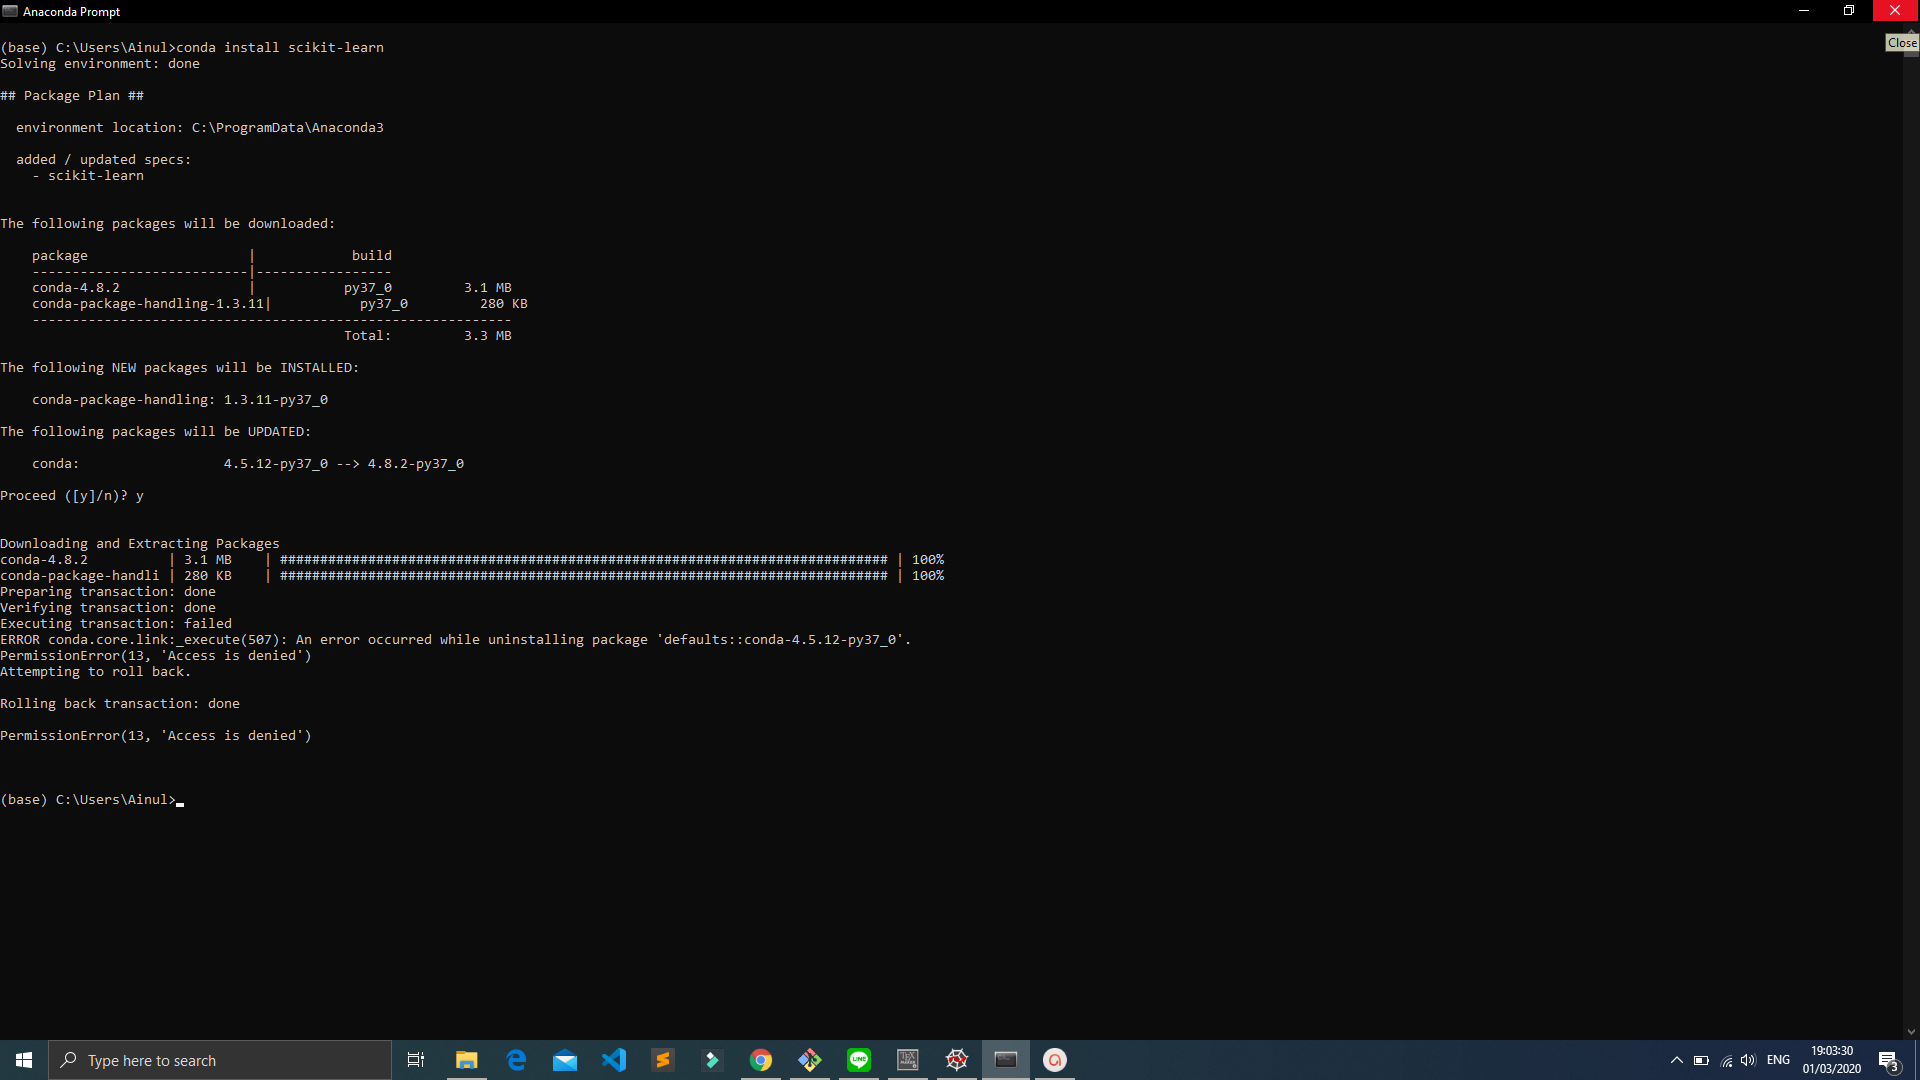
\includegraphics[width=4cm]{figures/1174073/1/1.png}
		\centering
		\caption{Instalasi Package Scikit Learn}
	\end{figure}
	\begin{figure}[H]
		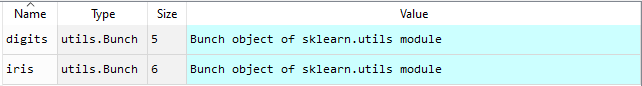
\includegraphics[width=4cm]{figures/1174073/1/2.png}
		\centering
		\caption{Isi Variabel Explorer}
	\end{figure}
	\item Mencoba Loading an example dataset, menjelaskan maksud dari tulisan tersebut dan mengartikan           		  per baris
	\hfill\break
	\lstinputlisting[firstline=7, lastline=11]{src/1174073/1/1174073.py}
	\item Mencoba Learning and predicting, menjelaskan maksud dari tulisan tersebut dan mengartikan per  			  baris
	\hfill\break
	\lstinputlisting[firstline=13, lastline=22]{src/1174073/1/1174073.py}
	\item  Mencoba Model persistence, menjelaskan maksud dari tulisan tersebut dan mengartikan per baris
	\hfill\break
	\lstinputlisting[firstline=25, lastline=34]{src/1174073/1/1174073.py}
	\item Mencoba Conventions, menjelaskan maksud dari tulisan tersebut dan mengartikan per baris
	\hfill\break
	\lstinputlisting[firstline=37, lastline=48]{src/1174073/1/1174073.py}
\end{enumerate}

\subsection{Penanganan Error}
\begin{enumerate}
	\item ScreenShoot Error
	\begin{figure}[H]
		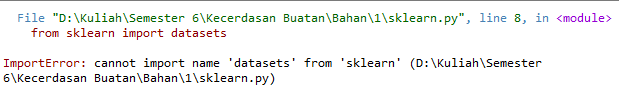
\includegraphics[width=4cm]{figures/1174073/1/error/1.png}
		\centering
		\caption{Import Error}
	\end{figure}

	\item Tuliskan Kode Error dan Jenis Error
	\begin{itemize}
		\item Import Error
	\end{itemize}
	\item Cara Penangan Error
	\begin{itemize}
		\item Import Error
		\hfill\break
		Dengan Menginstall Library Yang Tidak Ditemukan
	\end{itemize}
\end{enumerate}

\subsection{Bukti Tidak Plagiat}
\begin{figure}[H]
	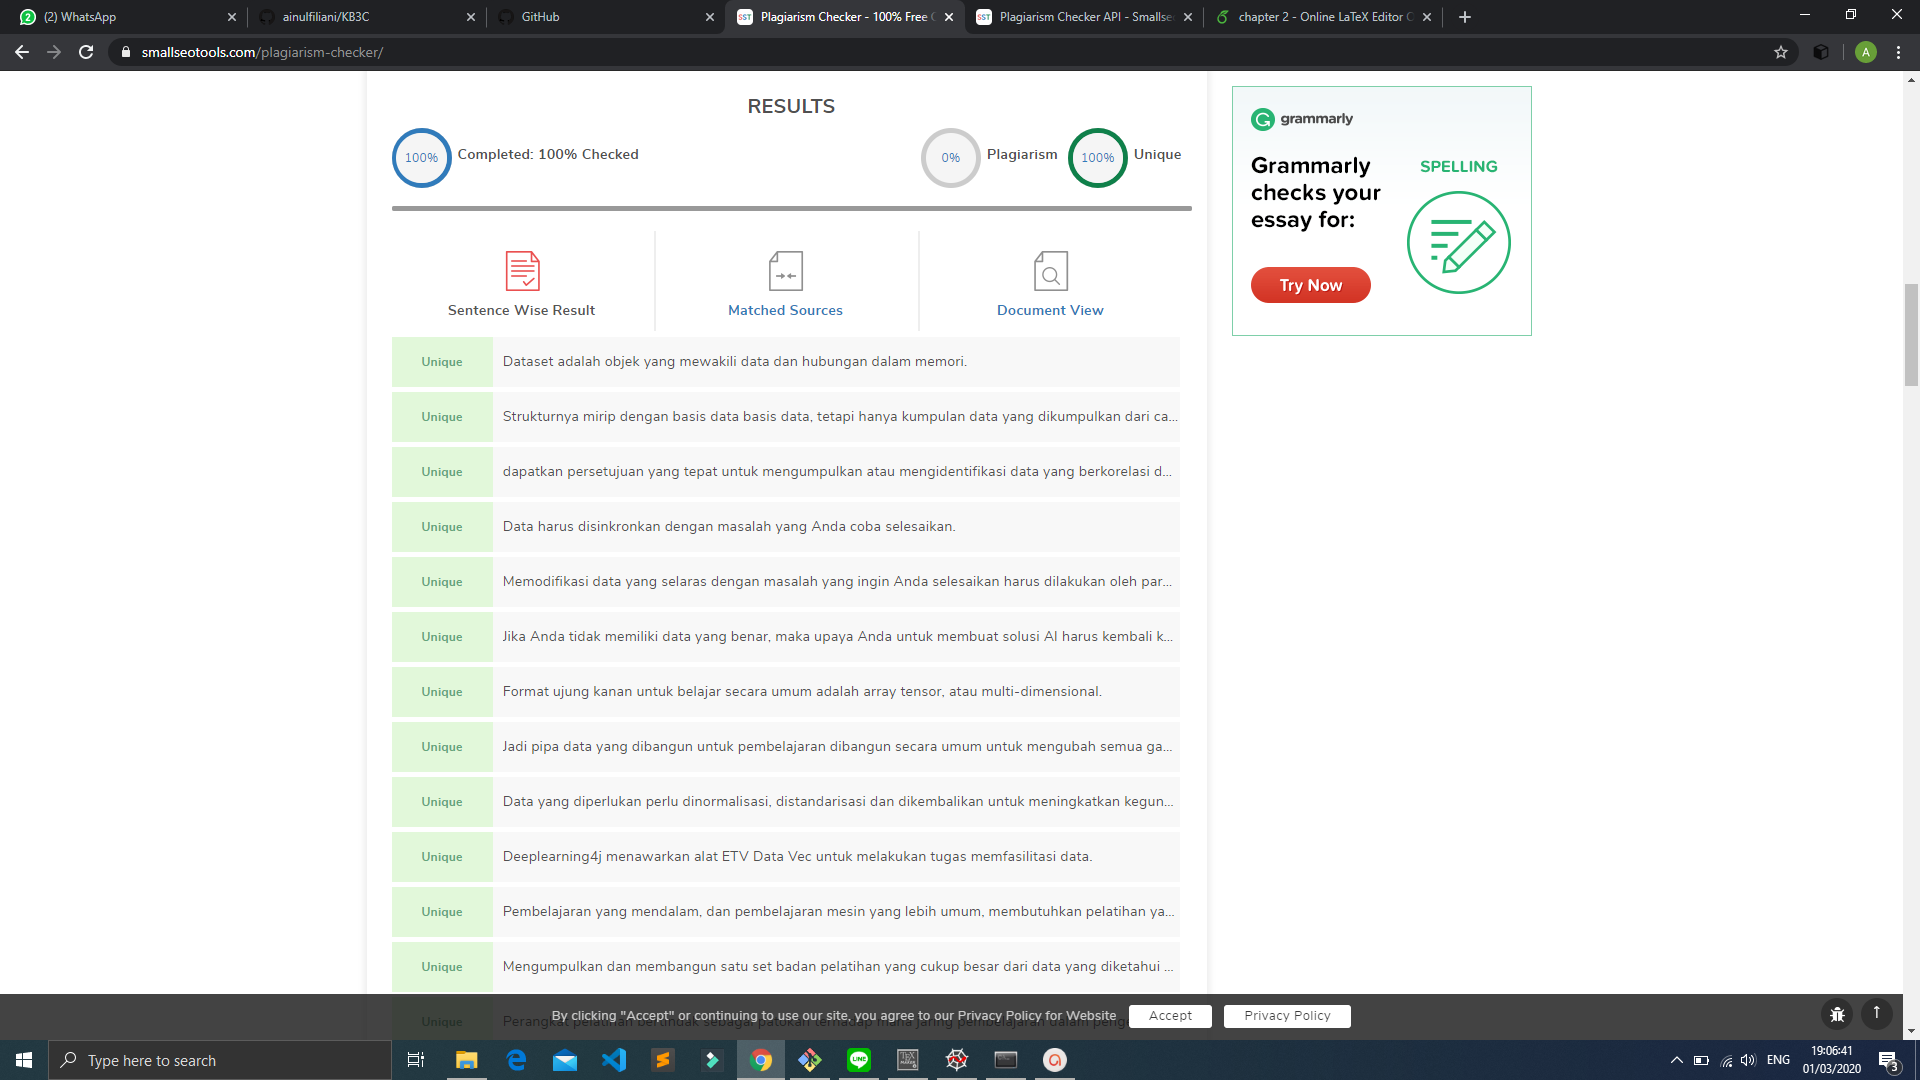
\includegraphics[width=4cm]{figures/1174073/1/plagiat/plagiat.png}
	\centering
	\caption{Bukti Tidak Melakukan Plagiat Chapter 1}
\end{figure}

\subsection{Link Youtube}


